%----------------------------------------------------------------------------
% Magic tutorial number 8
%----------------------------------------------------------------------------

\NeedsTeXFormat{LaTeX2e}[1994/12/01]
\documentclass[letterpaper,twoside,12pt]{article}
\usepackage{epsfig,times}

\setlength{\textwidth}{8.5in}
\addtolength{\textwidth}{-2.0in}
\setlength{\textheight}{11.0in}
\addtolength{\textheight}{-2.0in}
\setlength{\oddsidemargin}{0in}
\setlength{\evensidemargin}{0pt}
\setlength{\topmargin}{-0.5in}
\setlength{\headheight}{0.2in}
\setlength{\headsep}{0.3in}
\setlength{\topskip}{0pt}

\def\hinch{\hspace*{0.5in}}
\def\starti{\begin{center}\begin{tabbing}\hinch\=\hinch\=\hinch\=hinch\hinch\=\kill}
\def\endi{\end{tabbing}\end{center}}
\def\ii{\>\>\>}
\def\mytitle{Magic Tutorial \#8: Circuit Extraction}

%----------------------------------------------------------------------------

\begin{document}

\makeatletter
\newcommand{\ps@magic}{%
	\renewcommand{\@oddhead}{\mytitle\hfil\today}%
	\renewcommand{\@evenhead}{\today\hfil\mytitle}%
	\renewcommand{\@evenfoot}{\hfil\textrm{--{\thepage}--}\hfil}%
	\renewcommand{\@oddfoot}{\@evenfoot}}
\newcommand{\ps@mplain}{%
	\renewcommand{\@oddhead}{}%
	\renewcommand{\@evenhead}{}%
	\renewcommand{\@evenfoot}{\hfil\textrm{--{\thepage}--}\hfil}%
	\renewcommand{\@oddfoot}{\@evenfoot}}
\makeatother
\pagestyle{magic}
\thispagestyle{mplain}


\begin{center}
  {\bfseries \Large \mytitle} \\
  \vspace*{0.5in}
  {\itshape Walter Scott} \\
  \vspace*{0.5in}
   Special Studies Program \\
   Lawrence Livermore National Laboratory \\
   P.O. Box 808, L-270 \\
   Livermore, CA  94550 \\
  \vspace*{0.25in}
  {\itshape (Updated by others, too.)} \\
  \vspace*{0.25in}
  This tutorial corresponds to Magic version 7. \\
\end{center}
\vspace*{0.5in}

{\noindent\bfseries\large Tutorials to read first:}
\starti
   \> Magic Tutorial \#1: Getting Started \\
   \> Magic Tutorial \#2: Basic Painting and Selection \\
   \> Magic Tutorial \#4: Cell Hierarchies
\endi

{\noindent\bfseries\large Commands introduced in this tutorial:}
\starti
   \> :extract
\endi

{\noindent\bfseries\large Macros introduced in this tutorial:}

\starti
   {\itshape (none)}
\endi

{\bfseries Changes since Magic version 4:}

\starti
   \> New form of {\bfseries :extract unique} \\
   \> Path length extraction with {\bfseries :extract length} \\
   \> Accurate resistance extraction with {\bfseries :extresis} \\
   \> Extraction of well connectivity and substrate nodes \\
   \> Checking for global net connectedness in {\itshape ext2sim}~(1) \\
   \> New programs: {\itshape ext2spice}~(1) and {\itshape extcheck}~(1) \\
\endi

\section{Introduction}

This tutorial covers the use of Magic's
circuit extractor.
The extractor computes from the layout the information needed
to run simulation tools such as {\itshape crystal}~(1) and {\itshape esim}~(1).
This information includes the sizes and shapes of transistors,
and the connectivity, resistance, and parasitic capacitance of nodes.
Both capacitance to substrate and several kinds of internodal
coupling capacitances are extracted.

Magic's extractor is both incremental and hierarchical:
only part of the entire layout must be re-extracted after each change,
and the structure of the extracted
circuit parallels the structure of the layout being extracted.
The extractor produces a separate {\bfseries .ext} file
for each {\bfseries .mag} file in a hierarchical design.
This is in contrast to previous extractors, such as Mextra,
which produces a single {\bfseries .sim} file that represents
the flattened (fully-instantiated) layout.

Sections 2 through 4 introduce Magic's {\bfseries :extract} command
and some of its more advanced features.
Section 5 describes what information actually gets extracted, and
discusses limitations and inaccuracies.
Section 6 talks about extraction styles.
Although the hierarchical {\itshape ext}~(5) format fully describes the
circuit implemented by a layout, very few tools currently accept it.
It is normally necessary to flatten the extracted circuit using
one of the programs discussed in Section 7, such as {\itshape ext2sim}~(1),
{\itshape ext2spice}~(1), or {\itshape extcheck}~(1).

\section{Basic Extraction}

You can use Magic's extractor in one of several ways.
Normally it is not necessary to extract all cells in a layout.
To extract only those cells that have changed since they were extracted, use:

\starti
   \ii {\bfseries :load} {\itshape root} \\
   \ii {\bfseries :extract}
\endi

The extractor looks for a {\bfseries .ext} file for every cell in the tree
that descends from the cell {\itshape root}.
The {\bfseries .ext} file is searched for in the same directory that
contains the cell's {\bfseries .mag} file.
Any cells that have been modified since they were last extracted,
and all of their parents, are re-extracted.
Cells having no {\bfseries .ext} files are also re-extracted.

To try out the extractor on an example, copy all the {\bfseries tut8}{\itshape x}
cells to your current directory with the following shell commands:

\starti
   \ii {\bfseries cp \~{}cad/lib/magic/tutorial/tut8*.mag\ \ .}
\endi

Start magic on the cell {\bfseries tut8a} and type {\bfseries :extract}.
Magic will print the name of each cell ({\bfseries tut8a}, {\bfseries tut8b},
{\bfseries tut8c}, and {\bfseries tut8d}) as it is extracted.
Now type {\bfseries :extract} a second time.  This time nothing gets
printed, since Magic didn't have to re-extract any cells.
Now delete the piece of poly labelled ``{\bfseries delete me}''
and type {\bfseries :extract} again.  This time, only the cell
{\bfseries tut8a} is extracted as it is the only one that changed.
If you make a change to cell {\bfseries tut8b} (do it) and then
extract again, both {\bfseries tut8b} and {\bfseries tut8a} will be re-extracted,
since {\bfseries tut8a} is the parent of {\bfseries tut8b}.

To force all cells in the subtree rooted at cell {\itshape root}
to be re-extracted, use {\bfseries :extract\ all}:

\starti
   \ii {\bfseries :load}{\itshape  root} \\
   \ii {\bfseries :extract all}
\endi

Try this also on {\bfseries tut8a}.

You can also use the {\bfseries :extract} command to extract a single cell
as follows:

\starti
   \ii {\bfseries :extract cell} {\itshape name}
\endi

will extract just the selected (current) cell, and place the output
in the file {\itshape name}.
Select the cell {\bfseries tut8b} ({\bfseries tut8b{\_}0}) and type
{\bfseries :extract cell differentFile} to try this out.
After this command, the file {\bfseries differentFile.ext} will
contain the extracted circuit for the cell {\bfseries tut8b}.
The children of {\bfseries tut8b} (in this case, the single cell {\bfseries tut8d})
will not be re-extracted by this command.
If more than one cell is selected, the upper-leftmost one is extracted.

You should be careful about using {\bfseries :extract cell},
since even though you may only make a change to a child
cell, all of its parents may have to be re-extracted.
To re-extract all of the parents of the selected cell, you may use

\starti
   \ii {\bfseries :extract parents}
\endi

Try this out with {\bfseries tut8b} still selected.  Magic will extract
only the cell {\bfseries tut8a}, since it is the only one that uses the
cell {\bfseries tut8b}.
To see what cells would be extracted by {\bfseries :extract parents}
without actually extracting them, use

\starti
   \ii {\bfseries :extract showparents}
\endi

Try this command as well.

\section{Feedback: Errors and Warnings}

When the extractor encounters problems, it leaves feedback in the form
of stippled white rectangular areas on the screen.
Each area covers the portion of the layout that caused the error.
Each area also has an error message associated with it, which you can see
by using the {\bfseries :feedback} command.
Type {\bfseries :feedback help} while
in Magic for assistance in using the {\bfseries :feedback} command.

The extractor will always report extraction {\itshape errors}.
These are problems in
the layout that may cause the output of the extractor to be incorrect.
The layout should be fixed to eliminate extraction errors
before attempting to simulate the circuit; otherwise, the
results of the simulation may not reflect reality.

Extraction errors can come from violations of transistor rules.
There are two rules about the formation of transistors:
no transistor can be formed, and none can be destroyed,
as a result of cell overlaps.
For example, it
is illegal to have poly in one cell overlap diffusion in another cell,
as that would form a transistor in the parent where none was present
in either child.  It is also illegal to have a buried contact in one
cell overlap a transistor in another, as this would destroy the transistor.
Violating these transistor rules will cause design-rule violations
as well as extraction errors.
These errors only relate to circuit extraction: the fabricated
circuit may still work; it just won't be extracted correctly.

In general, it is an error for material of two types on the same plane
to overlap or abut if they don't connect to each other.  For example,
in CMOS it is illegal for p-diffusion and n-diffusion to overlap or abut.

In addition to errors, the extractor can give {\itshape warnings}.
If only warnings are present, the extracted circuit can still be
simulated.
By default, only some types of warnings are reported and displayed as feedback.
To cause all warnings to be displayed, use

\starti
   \ii {\bfseries :extract warn all}
\endi

The command

\starti
   \ii {\bfseries :extract warn} {\itshape warning}
\endi

may be used to enable specific warnings selectively; see below.
To cause no warnings to be displayed, or to disable display
of a particular {\itshape warning}, use respectively

\starti
   \ii {\bfseries :extract warn no all} or \\
   \ii {\bfseries :extract warn no} {\itshape warning}
\endi

Three different kinds of warnings are generated.
The {\bfseries dup} warning checks to see whether you
have two electrically unconnected nodes in the same
cell labelled with the same name.
If so, you are warned because the two unconnected
nodes will appear to be connected in the resulting {\bfseries .ext} file,
which means that the extracted circuit would not represent the actual layout.
This is bad if you're simulating the circuit to see if it will work
correctly: the simulator will think the two nodes are connected,
but since there's no physical wire between them, the electrons won't!
When two unconnected nodes share the same label (name), the extractor leaves
feedback squares over each instance of the shared name.

It's an excellent idea to avoid labelling two unconnected nodes with the same
name within a cell.  Instead, use the "correct" name for one of the
nodes, and some mnemonic but textually distinct name for the other nodes.
For example, in a cell with multiple power rails, you might use
{\bfseries Vdd!} for one of the rails, and names like {\bfseries Vdd\#1} for the
others.  As an example, load the cell {\bfseries tut8e}.
If the two nodes are connected in a higher-level cell
they will eventually be merged when the extracted circuit is flattened.
If you want to simulate a cell out
of context, but still want the higher-level nodes to be hooked up,
you can always create a dummy parent cell that hooks them together,
either with wire or by using the same name for pieces of paint that
lie over the terminals to be connected; see the cell {\bfseries tut8f}
for an example of this latter technique.

You can use the command

\starti
   \ii {\bfseries :extract unique}
\endi

as an automatic means
of labelling nodes in the manner described above.  Run this command on
the cell {\bfseries tut8g}.  A second version of this command is provided
for compatibility with previous versions of Magic.
Running

\starti
   \ii {\bfseries :extract unique \#}
\endi

will only 
append a unique numeric suffix to labels that end with a ``{\bfseries \#}''.
Any other duplicate nodenames that also don't end in a ``{\bfseries !}''
(the global nodename suffix as described in Section 5)
are flagged by feedback.  

A second type of warning, {\bfseries fets}, checks to see whether any transistors
have fewer diffusion terminals than the minimum for their types.
For example, the transistor type ``{\bfseries dfet}'' is defined in
the {\bfseries nmos} technology file as requiring two diffusion terminals:
a source and a drain.
If a capacitor with only one diffusion terminal is desired in this
technology, the type {\bfseries dcap} should be used instead.
The {\bfseries fets} warning is a consistency check for transistors
whose diffusion terminals have been accidentally shorted together,
or for transistors with insufficiently many diffusion terminals.

The third warning, {\bfseries labels},
is generated if you violate the following
guideline for placement of labels:
Whenever geometry from two subcells abuts or overlaps,
it's a good idea to make sure that
there is a label attached to the geometry in each subcell
{\itshape in the area of the overlap or along the line of abutment}.
Following this guideline isn't necessary for the extractor to work,
but it will result in noticeably faster extraction.

By default, the {\bfseries dup} and {\bfseries fets} warnings are enabled,
and the {\bfseries labels} warning is disabled.

Load the cell {\bfseries tut8h}, expand all its children ({\bfseries tut8i} and
{\bfseries tut8j}), and enable
all extractor warnings with {\bfseries :extract warn all}.
Now extract {\bfseries tut8h} and all of its children with
{\bfseries :extract}, and examine the feedback for examples of
fatal errors and warnings.

\section{Advanced Circuit Extraction}

\subsection{Lengths}

The Magic extractor has a rudimentary ability to compute wire lengths
between specific named points in a circuit.  This feature is intended for
use with technologies where the wire length between two points is
more important than the total capacitance on the net; this may
occur, for example, when extracting circuits with very long wires
being driven at high speeds ({\itshape e.g.}, bipolar circuits).
Currently, you must indicate to Magic which pairs of points are
to have distances computed.  You do this by providing two lists:
one of {\itshape drivers} and one of {\itshape receivers}.  The extractor
computes the distance between each driver and each receiver
that it is connected to.

Load the cell {\bfseries tut8k}.  There are five labels: two are drivers
({\bfseries driver1} and {\bfseries driver2}) and three are receivers
({\bfseries receiverA}, {\bfseries receiverB}, and {\bfseries receiverC}).
Type the commands:

\starti
   \ii {\bfseries :extract length driver driver1 driver2} \\
   \ii {\bfseries :extract length receiver receiverA receiverB receiverC}
\endi

Now enable extraction of lengths with {\bfseries :extract do length}
and then extract the cell ({\bfseries :extract}).
If you examine {\bfseries tut8k.ext}, you will see several {\bfseries distance}
lines, corresponding to the driver-receiver distances described
above.  These distances are through the centerlines of wires
connecting the two labels; where multiple paths exist, the
shortest is used.

Normally the driver and receiver tables will be built by using
{\bfseries :source} to read a file of {\bfseries :extract length driver}
and {\bfseries :extract length receiver} commands.  Once these tables
are created in Magic, they remain until you leave Magic or type
the command

\starti
   \ii {\bfseries :extract length clear}
\endi

which wipes out both tables.

Because extraction of wire lengths is {\itshape not} performed hierarchically,
it should only be done in the root cell of a design.  Also, because
it's not hierarchical, it can take a long time for long, complex wires such
as power and ground nets.  This feature is still experimental and
subject to change.

\subsection{Resistance}

Magic provides for more accurate resistance extraction using the
{\bfseries :extresis }command. {\bfseries :extresis} provides a detailed
resistance/capacitance
description for nets where parasitic resistance is likely to significantly
affect circuit timing.  

\subsubsection{Tutorial Introduction}

To try out the resistance extractor, load in the cell {\bfseries tut8r}.  Extract it
using {\bfseries :extract}, pause magic, and run ext2sim on the cell with the command

\starti
   \ii {\bfseries ext2sim tut8r}  
\endi

This should produce {\bfseries tut8r.sim}, {\bfseries tut8r.nodes}, 
and {\bfseries tut8r.al}. Restart magic and type  

\starti
   \ii {\bfseries :extresis tolerance 10} \\
   \ii {\bfseries :extresis}
\endi

This will 
extract interconnect resistances for any net where the interconnect delay 
is at least one-tenth of the transistor delay.  Magic should give the messages:

\starti
   \ii {\bfseries :extresis tolerance 10} \\
   \ii {\bfseries :extresis} \\
   \ii {\bfseries Adding  net2; Tnew = 0.428038ns,Told = 0.3798ns} \\
   \ii {\bfseries Adding  net1; Tnew = 0.529005ns,Told = 0.4122ns} \\
   \ii {\bfseries Total Nets: 7} \\
   \ii {\bfseries Nets extracted: 2 (0.285714)} \\
   \ii {\bfseries Nets output: 2 (0.285714)}
\endi

These may vary slightly depending on your technology parameters.
The {\bfseries Adding [net]} lines describe which networks for which magic produced 
resistor networks.  {\bfseries Tnew} is the estimated delay on the net including the
resistor parasitics, while {\bfseries Told} is the delay without parasitics.  
The next line describes where magic thinks the slowest node in the net is.  
The final 3
lines give a brief summary of the total number of nets, the nets requiring
extraction, and the number for which resistors were added to the output.

Running the resistance extractor also produced the file {\bfseries cell.res.ext}.  To
produce a {\bfseries .sim} file containing resistors, quit magic and type:

\starti
   \ii {\bfseries cat tut8r.ext tut8r.res.ext $>$tut8r.2.ext} \\
   \ii {\bfseries ext2sim -R -t! -t\# tut8r.2}
\endi

Comparing the two files, {\bfseries tut8r.sim} and {\bfseries tut8r.2.sim}, shows
that the latter has the nodes net1 and net2 split into several parts, with
resistors added to connect the new nodes together.

\subsubsection{General Notes on using the resistance extractor}

To use {\bfseries :extresis}, the circuit must first be extracted using
{\bfseries :extract} and flattened using ext2sim. When ext2sim is run,
do not use the {\bfseries -t\#} and {\bfseries -t!} flags (i.e. don't
trim the trailing "\#" and "!" characters) or the {\bfseries -R} flag
because {\bfseries :extresis} needs the {\bfseries .sim} and {\bfseries .ext}
names to correspond exactly, and it needs the lumped resistance values that
the extractor produces. Also, do not delete or rename the {\bfseries .nodes}
file; {\bfseries :extresis} needs this to run. Once the {\bfseries .sim} and
{\bfseries .nodes} files have been produced, type the command
{\bfseries :extresis} while running magic on the root cell.  As the
resistance extractor runs, it will identify which nets (if any) for
which it is producing RC networks, and will
identify what it thinks is the "slowest" point in the network.  When it
completes, it will print a brief summary of how many nets it extracted and
how many required supplemental networks.  The resistance networks are placed
in the file {\bfseries root.res.ext}.  To produce a {\bfseries .sim} file
with the supplemental
resistors, type {\bfseries cat root.ext root.res.ext $>$newname.ext}, and then rerun
{\bfseries ext2sim} on the new file.  During this second {\bfseries ext2sim} run, the 
{\bfseries -t} flag may be used.

Like extraction of wire lengths, resistance extraction is {\itshape not} performed 
hierarchically; it should only be done in the root cell of a design and
can take a long time for complex wires.

\subsubsection{Options, Features, Caveats and Bugs}

The following is a list of command line options and the arguments that they
take.

\begin{itemize}
   \item {\bfseries tolerance [value]} \\ This controls how large the
	resistance in a network must be before it is added to the
	output description. {\bfseries value} is defined as the minimum
	ratio of transistor resistance to interconnect resistance that
	requires a resistance network.  The default value is 1; values
	less than 1 will cause fewer resistors to be output and will make
	the program run faster, while values greater than 1 will produce
	more a larger, more accurate description but will  run slower.

   \item {\bfseries all} \\ Causes all nets in the circuit to be extracted;
	no comparison between transistor size and lumped resistance is
	performed.  This option is not recommended for large designs.

   \item {\bfseries simplify [on/off]} \\ Turns on/off the resistance network
	simplification routines.  Magic normally simplifies the resistance
	network it extracts by removing small resistors; specifying this flag
	turns this feature off.

   \item {\bfseries extout [on/off]} \\ Turns on and off the writing of the
	{\ttfamily root.res.ext} file.  The default value is on.

   \item {\bfseries lumped [on/off]} \\ Turns on the writing of
	{\ttfamily root.res.lump}.  This file contains an updated
	value of the lumped resistance for each net that
	{\bfseries :extresis} extracts.  

   \item {\bfseries silent [on/off]} \\ This option suppresses printing
	of the name and location of nets for which resistors are produced.

   \item {\bfseries skip mask} \\ Specifies a list of layers that the
	resistance extractor is to ignore.

   \item {\bfseries help} \\ Print brief list of options.
\end{itemize}

Attribute labels may also be used to specify certain extractor options.  For
a description of attributes and how they work, see tutorial 2.  Following is
a description of {\bfseries :extresis} attributes.

\begin{itemize}
   \item {\bfseries res:skip@} \\
	Causes this net to be skipped.  This is useful for avoiding
	extraction of power supplies or other DC signals that are not
	labeled Vdd or GND.

   \item {\bfseries res:force@} \\
	Forces extraction of this net regardless of its lumped
	resistance value.  Nets with both skip and force labels attached
	will cause the extractor to complain.

   \item {\bfseries res:min=[value]@} \\ Sets the smallest resistor size
	for this net.  The default value is the resistance of the largest
	driving transistor divided by the tolerance described above.

   \item {\bfseries res:drive@} - Nets with no driving transistors will normally
	not be extracted.  This option allows the designer to specify from
	where in the net the signal is driven.  This is primarily useful
	when extracting subcells, where the transistors driving a given signal
	may be located in a different cell.
\end{itemize}

\subsubsection{Technology File Changes}

Certain changes must be made in the extract section of the technology file
to support resistance extraction.  These include the {\bfseries fetresist} and {\bfseries contact}
lines, plus a small change to the fet line. Full details can be found in
Magic Maintainer's Manual \#2.  The only thing to note is that, contrary to
the documentation, the {\bfseries gccap} and {\bfseries gscap} parts of the fet line MUST 
be set; the resistance extractor uses them to calculate RC time constants for
the circuit.

\section{Extraction Details and Limitations}

This section explores in greater depth what gets extracted by Magic,
as well as the limitations of the circuit extractor.
A detailed explanation of the format of the {\bfseries .ext} files
output by Magic may be found in the manual page {\itshape ext}~(5).
``Magic Maintainer's Manual\ \#2: The Technology File''
describes how extraction parameters are specified for the extractor.

\begin{figure}[ht]
   \begin{center}
      \epsfig{file=../psfigures/tut8.1.ps, width=0.33\columnwidth}
      \caption{Each node extracted by Magic has a lumped resistance
	{\itshape R} and a lumped capacitance {\itshape C} to the
	substrate.  These lumped values can be interpreted as in the
	diagram above, in which each device connected to the node is
	attached to one of the points {\itshape 1}, {\itshape 2},
	\dots, {\itshape N}.}
   \end{center}
\end{figure}

\subsection{Nodes}

Magic approximates the pieces of interconnect between transistors
as ``nodes''.  A node is like an equipotential region, but
also includes a lumped resistance and capacitance to substrate.
Figure 1 shows how these lumped values are intended to be interpreted by
the analysis programs that use the extracted circuit.

Each node in an extracted circuit has a name, which is either
one of the labels attached to the geometry in the node if any exist,
or automatically generated by the extractor.  These latter names
are always of the form {\itshape p{\_}x{\_}y\#}, where
{\itshape p}, {\itshape x}, and {\itshape y} are integers,
{\itshape e.g.}, {\bfseries 3{\_}104{\_}17\#}.
If a label ending in the character ``{\bfseries !}'' is attached to a
node, the node is considered to be a ``global''.  Post-processing
programs such as {\itshape ext2sim}~(1) will check to ensure that
nodes in different cells that are labelled with the same global
name are electrically connected.

Nodes may have attributes attached to them as well as names.
Node attributes are labels ending in the special character
``{\bfseries @}'', and provide a mechanism for passing information
to analysis programs such as {\itshape crystal}~(1).  The man
page {\itshape ext}~(5) provides additional information about
node attributes.

\subsection{Resistance}

Magic extracts a lumped resistance for each node, rather than a
point-to-point resistance between each pair of devices connected
to that node.  The result is that all such
point-to-point resistances are approximated by the
worst-case resistance between any two points in that node.

By default,
node resistances are approximated rather than computed exactly.
For a node comprised entirely of a single type of material,
Magic will compute the node's total perimeter and area.
It then solves a quadratic equation to find the width and height of a simple
rectangle with this same perimeter and area, and approximates the
resistance of the node as the resistance of this ``equivalent''
rectangle.  The resistance is always taken in
the longer dimension of the rectangle.
When a node contains more than a single type of material, Magic
computes an equivalent rectangle for each type, and then sums
the resistances as though the rectangles were laid end-to-end.

This approximation for resistance does not take into account any
branching, so it can be significantly in error for nodes that have
side branches.  Figure 2 gives an example.
For global signal trees such as clocks or power, Magic's estimate of
resistance will likely be several times higher than the actual
resistance between two points.

\begin{figure}[ht]
   \begin{center}
      \epsfig{file=../psfigures/tut8.2.ps, width=0.8\columnwidth}
      \caption{Magic approximates the resistance of a node by
	assuming that it is a simple wire.  The length and width
	of the wire are estimated from the node's perimeter and area.
	(a) For non-branching nodes, this approximation is a good one.
	(b) The computed resistance for this node is the same as for
	(a) because the side branches are counted, yet the actual
	resistance between points 1 and 2 is significantly less
	than in (a).}
   \end{center}
\end{figure}

The approximated resistance also does not lend itself well to
hierarchical adjustments, as does capacitance.  To allow programs
like {\bfseries ext2sim} to incorporate hierarchical adjustments into
a resistance approximation, each node in the {\bfseries .ext} file
also contains a perimeter and area for each ``resistance class''
that was defined in the technology file (see ``Maintainer's
Manual \#2: The Technology File,'' and {\itshape ext}~(5)).
When flattening a circuit, {\bfseries ext2sim} uses this information
along with adjustments to perimeter and area
to produce the value it actually uses for node resistance.

If you wish to disable the extraction of resistances and node
perimeters and areas, use
the command

\starti
   \ii {\bfseries :extract no resistance}
\endi

which will cause all node resistances, perimeters, and areas in
the {\bfseries .ext} file to be zero.
To re-enable extraction of resistance, use
the command

\starti
   \ii {\bfseries :extract do resistance}.
\endi

Sometimes it's important that resistances be computed more accurately
than is possible using the lumped approximation above.
Magic's {\bfseries :extresist} command does this by computing explicit
two-terminal resistors and modifying the circuit network to
include them so it reflects more exactly the topology of the layout.
See the section on {\bfseries Advanced Extraction} for more details
on explicit resistance extraction with {\bfseries :extresist}.

\begin{figure}[ht]
   \begin{center}
      \epsfig{file=../psfigures/tut8.3.ps, width=0.5\columnwidth}
      \caption{Each type of edge has capacitance to substrate per
	unit length.  Here, the diffusion-space perimeter of 13 units
	has one value per unit length, and the diffusion-buried perimeter
	of 3 units another.  In addition, each type of material has
	capacitance per unit area.}
   \end{center}
\end{figure}

\subsection{Capacitance}

Capacitance to substrate comes from two different sources.
Each type of material has a capacitance to substrate per unit area.
Each type of edge (i.e, each pair of types) has a capacitance
to substrate per unit length.  See Figure 3.
The computation of capacitance may be disabled with

\starti
   \ii {\bfseries :extract no capacitance}
\endi

which causes all
substrate capacitance values in the {\bfseries .ext} file
to be zero.  It may be re-enabled with

\starti
   \ii {\bfseries :extract do capacitance}.
\endi

Internodal capacitance comes from three sources, as shown in Figure 4.
When materials of two different types overlap, the capacitance to
substrate of the one on top (as determined by the technology) is
replaced by an internodal capacitance to the one on the bottom.
Its computation may be disabled with

\starti
   \ii {\bfseries :extract no coupling}
\endi

which will also cause the extractor to run 30\% to 50\% faster.
Extraction of coupling capacitances can be re-enabled with

\starti
   \ii {\bfseries :extract do coupling}.
\endi

\begin{figure}[ht]
   \begin{center}
      \epsfig{file=../psfigures/tut8.4.ps, width=0.75\columnwidth}
      \caption{Magic extracts three kinds of internodal coupling
	capacitance.  This figure is a cross-section (side view, not
	a top view) of a set of masks that shows all three kinds of
	capacitance.  {\itshape Overlap} capacitance is parallel-plate
	capacitance between two different kinds of material when they
	overlap.  {\itshape Sidewall} capacitance is parallel-plate
	capacitance between the vertical edges of two pieces of the
	same kind of material.  {\itshape Sidewall overlap} capacitance
	is orthogonal-plate capacitance between the vertical edge of one
	piece of material and the horizontal surface of another piece of
	material that overlaps the first edge.}
   \end{center}
\end{figure}

\begin{figure}[ht]
   \begin{center}
      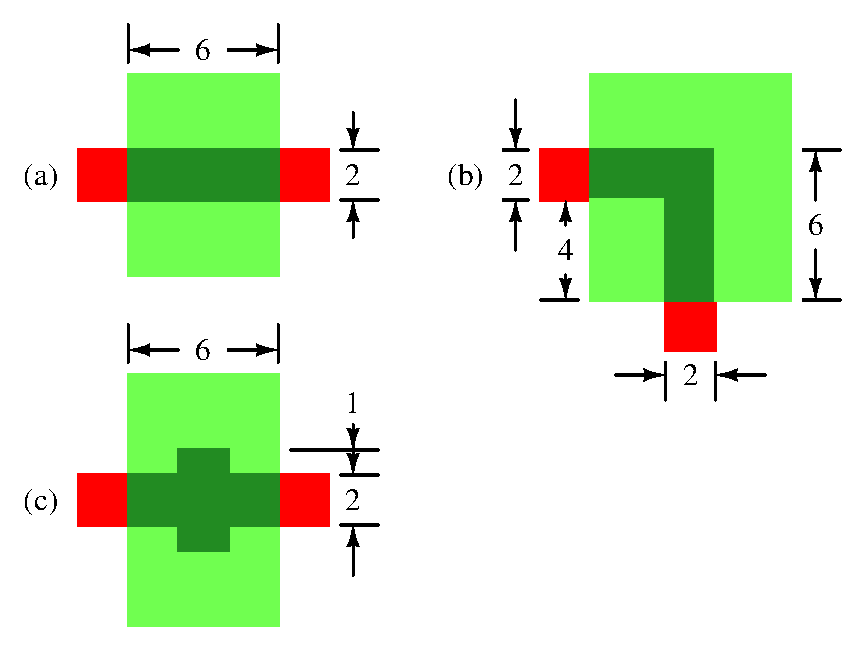
\epsfig{file=../psfigures/tut8.5.ps, width=0.75\columnwidth}
      \caption{
	(a) When transistors are rectangular, it is possible to
	compute $L / W$ exactly.  Here {\itshape gateperim}$=4$,
	{\itshape srcperim}$=6$, {\itshape drainperim}$=6$, and
	$L/W = 2/6$.
	(b) The $L/W$ of non-branching transistors can be approximated.
	Here {\itshape gateperim}$=4$, {\itshape srcperim}$=6$,
	{\itshape drainperim}$=10$.  By averaging {\itshape srcperim}
	and {\itshape drainperim} we get $L/W = 2/8$.
	(c) The $L/W$ of branching transistors is not well approximated.
	Here {\itshape gateperim}$=16$, {\itshape srcperim}$=2$,
	{\itshape drainperim}$=2$.  Magic's estimate of $L/W$ is $8/2$,
	whereas in fact because of current spreading, $W$ is effectively
	larger than $2$ and $L$ effectively smaller than $8$, so $L/W$ is
	overestimated.}
   \end{center}
\end{figure}

Whenever material from two subcells overlaps or abuts, the extractor
computes adjustments to substrate capacitance, coupling
capacitance, and node perimeter and area.  Often, these adjustments
make little difference to the type of analysis you are performing,
as when you wish only to compare netlists.  Even when running
Crystal for timing analysis, the adjustments can make less than
a 5\% difference in the timing of critical paths in designs with
only a small amount of inter-cell overlap.
To disable the computation of these adjustments, use

\starti
   \ii {\bfseries :extract no adjustment}
\endi

which will result in
approximately 50\% faster extraction.  This speedup is
not entirely additive with the speedup resulting from
{\bfseries :extract no coupling}.  To re-enable computation of adjustments, use
{\bfseries :extract do adjustment}.

\subsection{Transistors}

Like the resistances of nodes, the lengths and widths of transistors are
approximated.  Magic computes the contribution to the total perimeter
by each of the terminals of the transistor.  See Figure 5.
For rectangular transistors, this yields an exact \$L / W\$.
For non-branching, non-rectangular transistors, it is still
possible to approximate \$L / W\$ fairly well, but substantial
inaccuracies can be introduced if the channel of a transistor contains
branches.
Since most transistors are rectangular, however, Magic's approximation
works well in practice.

\begin{table}[ht]
   \begin{center}
      \begin{tabular}{|ccccccc|} \hline
	Type 	 & Loc         &  A  P & Subs & Gate & Source & Drain \\ \hline
	fet nfet & 59  1 60  2 &  8 12 & GND! & Mid2 4 {\bfseries N3}
		& Out 4 0    & Vss\#0 4 0 \\
	fet nfet & 36  1 37  2 &  8 12 & Float & Mid1 4 {\bfseries N2}
		& Mid2 4 0   & Vss\#0 4 0 \\
	fet nfet &  4  1  5  2 &  8 12 & Vss\#0 & In 4 {\bfseries N1}
		& Mid1 4 0   & Vss\#0 4 0 \\
	fet pfet & 59 25 60 26 &  8 12 & Vdd! & Mid2 4 {\bfseries P3}
		& Vdd\#0 4 0 & Out 4 0 \\
	fet pfet & 36 25 37 26 &  8 12 & VBias & Mid1 4 {\bfseries P2}
		& Vdd\#0 4 0 & Mid2 4 0 \\
	fet pfet &  4 25  5 26 &  8 12 & Vdd\#0 & In 4 {\bfseries P1}
		& Vdd\#0 4 0 & Mid1 4 0 \\ \hline
      \end{tabular}
      \caption{The transistor section of {\bfseries tut8l.ext}.}
   \end{center}
\end{table}

In addition to having gate, source, and drain terminals, MOSFET
transistors also have a substrate terminal.  By default,
this terminal is connected to a global node that depends
on the transistor's type.  For example, p-channel transistors
might have a substrate terminal of {\bfseries Vdd!}, while n-channel
transistors would have one of {\bfseries GND!}.
However, when a transistor is surrounded by explicit ``well'' material
(as defined in the technology file), Magic will override the
default substrate terminal with the node to which the well
material is connected.  This has several advantages: it allows
simulation of analog circuits in which wells are biased to
different potentials, and it provides a form of checking
to ensure that wells in a CMOS process are explicitly tied
to the appropriate DC voltage.

Transistor substrate nodes are discovered by the extractor only if
the transistor and the overlapping well layer are in the same cell.
If they appear in different cells, the transistor's substrate terminal
will be set to the default for the type of transistor.

Load the cell {\bfseries tut8l}, extract it, and look at the file
{\bfseries tut8l.ext}.  Table 1 shows the lines for the six
transistors in the file.  You'll notice that the substrate terminals
(the {\itshape Subs} column) for all transistors are different.
Since each transistor in this design has a different gate attribute attached
to it (shown in bold in the table, {\itshape e.g.}, {\bfseries N1},
{\bfseries P2}, etc), we'll use them in the following discussion.

The simplest two transistors are {\bfseries N3} and {\bfseries P3}, which don't
appear in any explicitly drawn wells.  The substrate terminals for
these are {\bfseries GND!} and {\bfseries Vdd!} respectively, since that's what
the technology file says is the default for the two types of transistors.
{\bfseries N1} and {\bfseries P1} are standard transistors that lie in wells tied
to the ground and power rails, labelled in this cell as {\bfseries Vss\#0}
and {\bfseries Vdd\#0} respectively.  (They're not labelled {\bfseries GND!} and
{\bfseries Vdd!} so you'll see the difference between {\bfseries N1} and {\bfseries N3}).
{\bfseries P2} lies in a well that is tied to a different bias voltage,
{\bfseries VBias}, such as might occur in an analog design.
Finally, {\bfseries N2} is in a well that isn't tied to any wire.
The substrate node appears as {\bfseries Float} because that's the label that
was attached to the well surrounding {\bfseries N2}.

The ability to extract transistor substrate nodes allows you to perform
a simple check for whether or not transistors are in properly connected
({\itshape e.g.}, grounded) wells.  In a p-well CMOS process, for example, you
might set the default substrate node for n-channel transistors to be
some distinguished global node other than ground, {\itshape e.g.},
{\bfseries NSubstrateNode!}.  You could then extract the circuit, flatten
it using {\itshape ext2spice}~(1) (which preserves substrate nodes,
unlike {\itshape ext2sim}~(1) which ignores them), and
look at the substrate node fields of all the n-channel transistors:
if there were any whose substrate nodes weren't connected to {\bfseries GND!},
then these transistors appear either outside of any explicit well
(their substrate nodes will be the default of {\bfseries NSubstrateNode}),
or in a well that isn't tied to {\bfseries GND!} with a substrate contact.

\section{Extraction styles}

Magic usually knows several different ways to extract
a circuit from a given layout.
Each of these ways is called a {\itshape style}.
Different styles can be used to handle different
fabrication facilities, which may differ in the parameters
they have for parasitic capacitance and resistance.
For a scalable technology, such as the default {\bfseries scmos},
there can be a different extraction style for each scale factor.
The exact number and nature of the extraction styles is
described in the technology file that Magic reads when it starts.
At any given time, there is one current extraction style.

To print a list of the extraction styles available, type
the command

\starti
   \ii {\bfseries :extract style}.
\endi

The {\bfseries scmos} technology currently has the styles {\bfseries lambda=1.5}, 
{\bfseries lambda=1.0}, and {\bfseries lambda=0.6}, though this changes over time as
technology evolves.
To change the extraction style
to {\itshape style}, use the command

\starti
   \ii {\bfseries :extract style}{\itshape style}
\endi

Each style has a specific scale factor between Magic units and
physical units ({\itshape e.g.}, microns);  you can't use a
particular style with a different scale factor.  To change
the scalefactor, you'll have to edit the appropriate
style in the {\bfseries extract} section of the technology file.
This process is described in
``Magic Maintainer's Manual \#2: The Technology File.''

\section{Flattening Extracted Circuits}

Unfortunately, very few tools exist to
take advantage of the {\itshape ext}~(5) format
files produced by Magic's extractor.
To use these files for simulation
or timing analysis,
you will most likely need to convert them to a flattened
format, such as {\itshape sim}~(5) or {\itshape spice}~(5).

There are several programs for flattening {\itshape ext}~(5) files.
{\itshape Ext2sim}~(1) produces {\itshape sim}~(5) files suitable
for use with {\itshape crystal}~(1), {\itshape esim}~(1), or {\itshape rsim}~(1).
{\itshape Ext2spice}~(1) is used to produce {\itshape spice}~(5) files
for use with the circuit-level simulator {\itshape spice}~(1).
Finally, {\itshape extcheck}~(1) can be used to perform connectivity
checking and will summarize the number of flattened nodes,
transistors, capacitors, and resistors in a circuit.
All of these programs make use of a library known as
{\itshape extflat}~(3), so the conventions for each and the
checks they perform are virtually identical.  The documentation
for {\itshape extcheck} covers the options common to all of
these programs.

To see how {\itshape ext2sim} works, load the cell {\bfseries tut8n}
and expand all the {\bfseries tutm} subcells.
Notice how the {\bfseries GND!} bus is
completely wired, but the {\bfseries Vdd!} bus is in three
disconnected pieces.
Now extract everything with {\bfseries :extract}, then
exit Magic and run {\bfseries ext2sim tut8n}.
You'll see the following sort of output:

\ttfamily
\starti
   \> *** Global name Vdd! not fully connected: \\
   \> One portion contains the names: \\
   \> \> left/Vdd! \\
   \> The other portion contains the names: \\
   \> \> center/Vdd! \\
   \> I'm merging the two pieces into a single node, but you \\
   \> should be sure eventually to connect them in the layout. \\ \\

   \> *** Global name Vdd! not fully connected: \\
   \> One portion contains the names: \\
   \> \> left/Vdd! \\
   \> \> center/Vdd! \\
   \> The other portion contains the names: \\
   \> \> right/Vdd! \\
   \> I'm merging the two pieces into a single node, but you \\
   \> should be sure eventually to connect them in the layout. \\ \\

   \> Memory used: 56k
\endi
\rmfamily

The warning messages are telling you that the global name
{\bfseries Vdd!} isn't completely wired in the layout.  The flattener
warns you, but goes ahead and connects the pieces together
anyway to allow you to simulate the circuit as though it
had been completely wired.
The output of {\itshape ext2sim} will be three files:
{\bfseries tut8n.sim}, {\bfseries tut8n.al}, and {\bfseries tut8n.nodes};
see {\itshape ext2sim}~(1) or {\itshape sim}~(5) for more information
on the contents of these files.
``{\bfseries Magic Tutorial \#11:  Using RSIM with Magic}'' explains how to use the
output of {\itshape ext2sim} with the switch-level simulator,
{\itshape rsim}~(1).

\end{document}
